% ============================================================= BENCHMARK ==
\section{The benchmark}\label{sec:benchmark}

\subsection{Corridors, splits and network}
The release covers five corridor families in two districts, each with two directions (\cref{tab:corridors}).
Every panel ships mainline speed, flow and occupancy at five-minute resolution, on- and off-ramp counts, link
geometry, per-link triangular fundamental-diagram parameters, an LWR topology file, a path set and a weak path-flow
prior. The training split runs from 1 June 2030 to 28 February 2031 (273 days) and ships an unmasked copy of every
observation. Validation (March 2031, 31 days) and private (April 2031, 30 days) ship only the masked layer.

\begin{table}[h]
\centering\small
\caption{The ten directional panels, computed from the released network files. Paths equal $Z(Z-1)/2$ for $Z$
zones: one path per upstream-to-downstream zone pair. Task 2 excludes the two D12 I-405 panels.}\label{tab:corridors}
\begin{tabular}{@{}l r r r r r r r@{}}
\toprule
Panel & Links & Length (km) & Detector links & Mean lanes & On / off ramps & Zones & Paths \\
\midrule
D7\_I10\_E    & 146 & 55.6 & 101 & 4.23 & 62 / 54 & 93 & 4,278 \\
D7\_I10\_W    & 107 & 49.1 & 107 & 4.17 & 60 / 55 & 101 & 5,050 \\
D7\_I210\_E   & 297 & 81.3 & 75  & 4.04 & 56 / 42 & 73 & 2,628 \\
D7\_I210\_W   & 81  & 44.5 & 81  & 3.99 & 62 / 45 & 82 & 3,321 \\
D7\_I405\_N   & 352 & 67.2 & 96  & 4.46 & 61 / 42 & 96 & 4,560 \\
D7\_I405\_S   & 109 & 42.0 & 109 & 4.35 & 62 / 51 & 97 & 4,656 \\
D12\_I5\_N    & 258 & 72.6 & 93  & 4.71 & 63 / 49 & 93 & 4,278 \\
D12\_I5\_S    & 100 & 45.0 & 100 & 4.67 & 53 / 54 & 101 & 5,050 \\
D12\_I405\_N  & 89  & 45.3 & 50  & 5.05 & 31 / 23 & 43 & 903 \\
D12\_I405\_S  & 44  & 32.7 & 44  & 5.02 & 27 / 20 & 36 & 630 \\
\midrule
Total         & 1,583 & 535.2 & 856 & & 537 / 435 & & 35,354 \\
\bottomrule
\end{tabular}
\end{table}

\Cref{fig:fd} shows the released diagrams. Jam density is exactly 100 veh/km/lane on every link; free-flow speeds
lie between 105 and 128 km/h, per-lane capacities mostly between 1,450 and 2,750 veh/h, and the implied backward
wave speed $w$ is about 23 km/h in District 7 and 26 km/h in District 12. Links are short: the shortest is 10 m and
many are a few hundred metres, so a five-minute bin is long compared with the free-flow travel time of a link.

\begin{figure}[t]
\centering
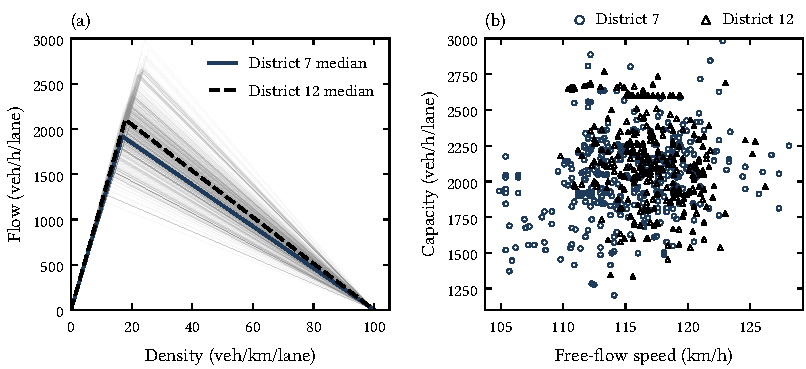
\includegraphics[width=\linewidth]{figures/fig_fundamental_diagram.pdf}
\caption{The physics the evaluator uses. Left: the per-lane triangular diagram of every link (grey) and the
median diagram of each district. Right: free-flow speed against per-lane capacity. Task 3 checks the submitted
speed and flow against these diagrams and against vehicle conservation.}\label{fig:fd}
\end{figure}

\subsection{Masking and eligibility}
A cell is \emph{eligible} when its detector reported for at least 75\,\% of the interval and the required values are
present; about 76\,\% of cells qualify, and only eligible cells are scored in any task. Task 1 removes eligible
cells under three regimes, R1, R2 and R3, at 20, 30 and 50\,\% of cells. Each calendar day belongs to exactly one
regime, so no cell hidden in one view is visible in another. At a blanked cell every measured channel is removed:
speed, flow, occupancy and the occupancy-derived density. The quality flag (\code{pct\_observed}) stays, so the
target cells are known. The Task 2 horizon and the 60 minutes after it are also blanked so that the horizon cannot
be interpolated across.

\subsection{Tasks and scoring}
\paragraph{Task 1, state} For each regime $r$, speed and per-lane flow errors are scored separately and blended,
\begin{equation}
  \begin{aligned}
  \Sstate(r) &= 0.54\,\max\!\Big(0,\,1-\frac{\mathrm{RMSE}_v(r)}{25\ \mathrm{km/h}}\Big)
              + 0.46\,\max\!\Big(0,\,1-\frac{\mathrm{RMSE}_{q/\mathrm{lane}}(r)}{600\ \mathrm{veh/h}}\Big),\\
  \Sstate &= \tfrac13\textstyle\sum_{r\in\{R1,R2,R3\}} \Sstate(r).
  \end{aligned}
  \label{eq:state}
\end{equation}
The equal weight on regimes means the 50\,\% mask counts as much as the 20\,\% mask.

\paragraph{Task 2, queue} A link is \emph{queued} when its latent speed is at most $0.6\,v_f$. Each window provides
the history up to the forecast origin $T$ and asks for the queue field $\hat Y\in\{0,1\}^{L\times 6}$ at
$T{+}5,\dots,T{+}30$ minutes. A window is scored by space-time intersection over union \cite{jaccard1912},
\begin{equation}
  \IoU(\hat Y, Y) = \frac{|\hat Y \wedge Y|}{|\hat Y \vee Y|},
  \label{eq:iou}
\end{equation}
and $\Squeue$ is the mean over windows, five \emph{onset} and five \emph{ongoing} per panel and split. Onset windows
have no queued link anywhere in the history and at least one in the horizon; ongoing windows have a queue at $T$.
Because the two conditions have equal counts, $0.30\,\Squeue = 0.15\,\IoU_{\mathrm{onset}} + 0.15\,\IoU_{\mathrm{ongoing}}$.

\paragraph{Task 3, physics} There are no Task 3 rows. The evaluator forms $k=q/v$ and $N=kL$ from the submitted state
and scores
\begin{equation}
  \Sphys = \tfrac13\,\SFD + \tfrac23\,\SLWR,
  \qquad
  N_{t+\Delta t}-N_t \overset{!}{=} \Delta t\,\big(q_{\mathrm{in}} + q_{\mathrm{on}} - q_{\mathrm{out}} - q_{\mathrm{off}}\big),
  \label{eq:phys}
\end{equation}
where $\SFD$ measures the normalized distance between the submitted flow and the diagram flow at the same density
\cite{lighthill1955,richards1956}, and $\SLWR$ the size of the conservation residual over link-to-link transitions
with the released ramps. All ten corridors use coverage mode A (0.756 ramp coverage).

\paragraph{Task 4, demand} With path-link incidence $A$, released counts $c$ and prior $b$,
$\Sodme = 0.45\,S_{\mathrm{od}} + 0.25\,S_{\mathrm{link}} + 0.15\,S_{\mathrm{dev}} + 0.15\,S_{\mathrm{attr}}$ compares
the submitted path flows $f$ to a withheld reference, $Af$ to $c$, the distance moved from $b$ to the reference's,
and the destination-attraction pattern.

\paragraph{Aggregation} Each component is computed per panel, the two directions of a corridor are averaged, and the
five corridor families are averaged with equal weight. A task with a missing or incomplete row set scores zero.

\subsection{Anatomy of a submission}
A submission has 6,980,503 rows: 6,735,795 \emph{state} rows (speed and flow for every Task 1 target cell of
validation and private), 174,000 \emph{queue} rows (8 panels $\times$ 10 windows $\times$ 1,450 links $\times$ 6
horizons, summed over two splits, half onset and half ongoing) and 70,708 \emph{ODME} rows (35,354 paths $\times$ 2
splits). This arithmetic matters for the analysis in \cref{sec:leaderboard}: the three blocks are disjoint, so each
task's score depends only on its own rows.

\subsection{Five properties of the design that shaped our method}\label{sec:design}
\begin{enumerate}[label=\textbf{P\arabic*.},leftmargin=2.2em]
  \item \textbf{Physics without lookup.} The generator obeys LWR-type physics with calibrated noise, but no external
        record contains the answers. Methods must model the release, not join against outside data.
  \item \textbf{Onsets are placed at the end of the horizon.} The onset selector takes the earliest qualifying
        origin, one whose hour of history has no queue and whose horizon does, with selected origins at least 360
        minutes apart. Simulating that rule on the training split reproduced 39 of the 40 published onset origins. A consequence is that the first queued
        cell almost always appears at $T{+}30$, the last horizon step. The release notes that onsets are visible in
        advance: an hour before a queue forms the road runs at about 1.28 times its queue threshold, against 1.54
        times where none follows, and carries about 6,912 veh/h against 4,620.
  \item \textbf{Ongoing windows are those where persistence fails.} A window is kept only if copying the current
        queue forward scores an IoU of at most 0.9 on it. Trivial persistence is therefore weaker than on random
        congested windows by construction.
  \item \textbf{Queue scores are noisy.} The organizers report a per-window IoU standard deviation of 0.3752 on
        the persistence baseline; with five windows per condition and panel this is about 0.0126 of $\Stotal$ from
        window sampling alone. Validation and private queue scores can differ by that much with no change in skill.
  \item \textbf{Physics cannot be scored locally.} The conservation check needs the organizer's boundary flows,
        which are withheld. Estimating them from the submitted flows swamps the signal: the conservation signal is
        about 0.75\,\% of the vehicles on a link and that estimate is off by about 0.22\,\%, so a perfect answer on
        D12\_I5\_N scores 0.3305 locally and 0.9604 with the organizer flows.
\end{enumerate}

\begin{table}[h]
\centering\small
\caption{Organizer reference scores on the validation split, from the baseline table of the benchmark repository.
These values anchor the additive decomposition of \cref{sec:leaderboard}; our submission of the same baselines
scored 0.55343.}\label{tab:baselines}
\begin{tabular}{@{}l l r r@{}}
\toprule
Component & Naive baseline & Baseline score & Perfect answer \\
\midrule
$\Sstate$ & weekday $\times$ time-of-day historical mean & 0.6929 & 1.0000 \\
$\Squeue$ & persistence of the last history slot & 0.3017 & 1.0000 \\
$\Sphys$ & (inherits the state baseline) & 0.3549 & 0.9636 \\
$\Sodme$ & NNLS against TRAIN counts & 0.8359 & 1.0000 \\
\midrule
$\Stotal$ & & 0.5534 & 0.9945 \\
\bottomrule
\end{tabular}
\end{table}
